\documentclass{article}
\usepackage{fancyhdr,graphicx}
\setlength{\headheight}{15.2pt}
\pagestyle{fancy}
\begin{document}
\rhead{\fancyplain{}Page {\thepage}}
\lhead{\fancyplain{}Section {\thesection}}
\title{Bioinformatics Analysis of Effect of Hydrogen Peroxide on \emph{Beta vulgaris} Seeds}
\author{Vinay Hiremath}
\date{16 July 2012}
\maketitle
\section{Introduction}
	It has recently been found through preliminary experiments that various types of seeds of the species \emph{Beta vulgaris} germinate significantly more successfully when placed in a solution of 0.3\% hydrogen peroxide (H$_{2}$O$_{2}$) as opposed to a solution of pure water (H$_{2}$O). There is a noticeable difference in both germination time (shorter) and the percentage of seeds (higher) that are germinated after four days. It is likely that this change in success rates is a direct effect of a change in the genes being expressed by these seeds, and this phenomenon likely reflects the relative emergence potential of the varieties of sugar beet. After obtaining DNA sequences of the seeds in both the control and experimental group, I will attempt to use various bioinformatic tools in conjunction to arrive at a result that clearly expresses the specific DNA sequences that are expressed only in the experimental (H$_{2}$O$_{2}$) group.
\section{Hypothesis}
	As a result of the extensive procedure necessary to properly sequence the DNA of the trial groups, the limited data to be analyzed may be slightly lacking in scope. However, by comparing the genes only expressed in the experimental with annotated genomes for both \emph{Beta vulgaris} and other similar organisms, it is hopeful to maintain that the isolated expressed DNA sequences have similar listed roles in these genomes. Through this assimilation of previously gathered data, the expression of certain genes to affect the success rate of germination of the various seeds should become clear after extensive gene analysis.
\section{Methods}
	I will be using a large suite of bioinformatics tools, all of which are open-sourced under the GNU Public License as freely redistributable. Annotated genome data will becollected from sources such as the Basic Local Alignment Search Tool (BLAST), Arabidopsis Information Resource (TAIR), and the Kyoto Encyclopedia of Genes and Genomes (KEGG), among others.\\\\
	In order to first build an index for the sequence files so that they can be more easily indexed, I first needed to generate detailed quality reports, so I used the fastqc toolset. Next, I used a tool called \emph{bowtie2} as it enables strong compatibility with the assembly program I used, known as \emph{tophat}. Using this suite of programs, I was able to assemble the data I had gathered onto the *** genome, made by ***. After this, I was able to analyze the remaining assembled data sets using the cufflinks suite. Cufflinks generated transcript indexes of each data set for both H$_{2}$O and H$_{2}$O$_{2}$ of each seed variety. Next, cuffdiff was able to find the sections of each contig that was different between the experimental and control data sets while avoiding those similar between the seed variety data sets, which helped to eliminate extraneous results. To convert these contigs to actual sequences as represented in the RefBeet genome, I made a custom script that extracts the base sequences from the reference genome by applying the contig number and position given by cuffdiff. After these sequences were found and input into a text file, I submitted them to a large variety of BLAST databases as previously listed. The annotated databases output predicted roles of each difference between the control and experimental data sets.

\section{Raw Data}
\subsection{Sequence Output Information}
\begin{center}
MSR3 set in water: \\
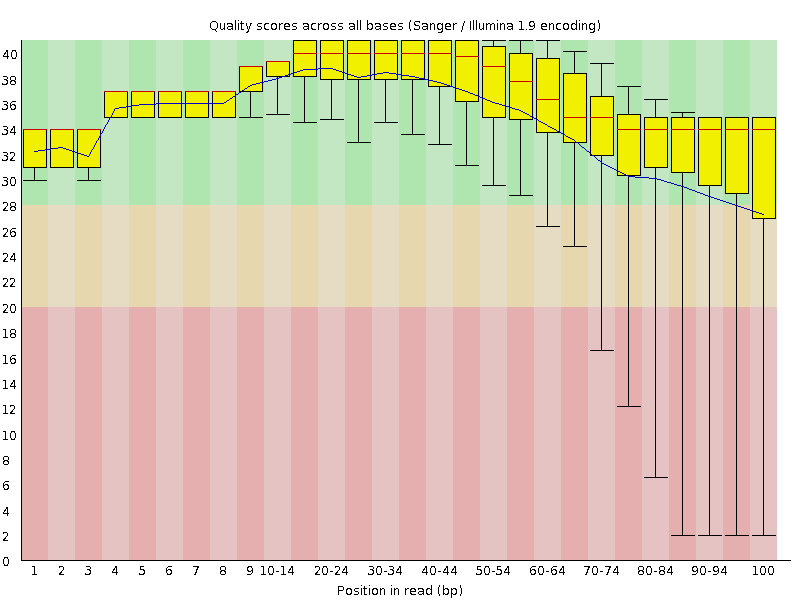
\includegraphics[scale=0.3]{msr3_h20_r1_basequal.png} \\
	\begin{tabular}{| l | r |}
	\hline
	Total sequences & 24155194 \\ \hline
	Sequence length & 100 \\ \hline
	\% GC content & 48 \\ \hline
	\end{tabular}

MSR3 set in hydrogen peroxide: \\
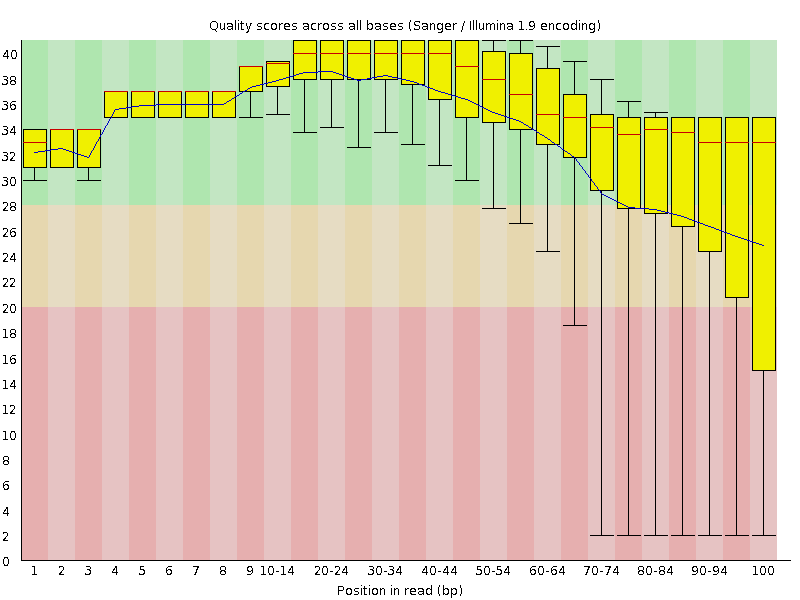
\includegraphics[scale=0.3]{msr3_h202_r1_basequal.png} \\
	\begin{tabular}{| l | r |}
	\hline
	Total sequences & 25694416 \\ \hline
	Sequence length & 100 \\ \hline
	\% GC content & 49 \\ \hline
	\end{tabular}
	
USH20 set in water: \\
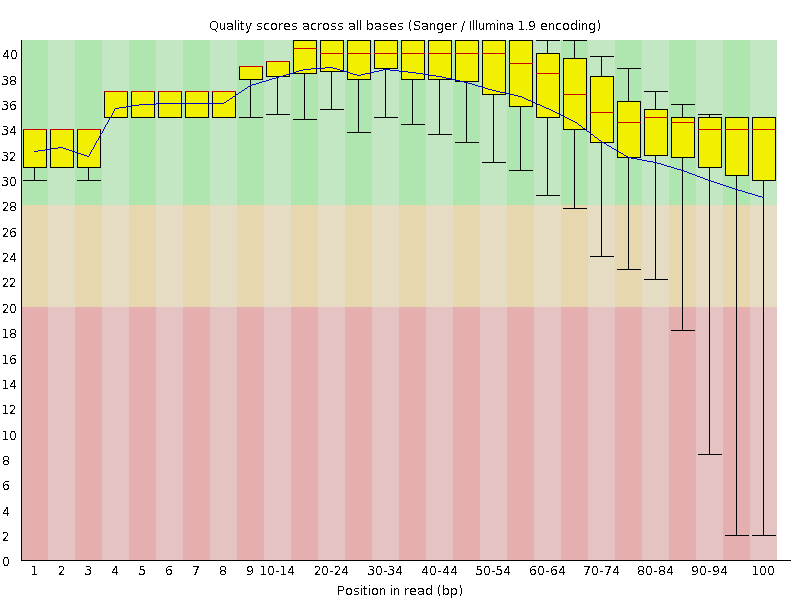
\includegraphics[scale=0.3]{ush20_h20_r1_basequal.png} \\
	\begin{tabular}{| l | r |}
	\hline
	Total sequences & 28485306 \\ \hline
	Sequence length & 100 \\ \hline
	\% GC content & 44 \\ \hline
	\end{tabular}

USH20 set in hydrogen peroxide: \\
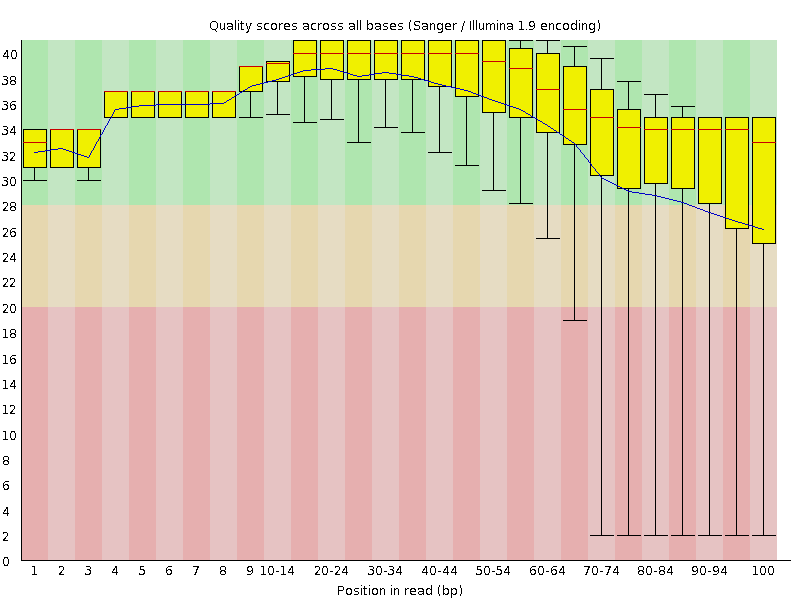
\includegraphics[scale=0.3]{ush20_h202_r1_basequal.png} \\
	\begin{tabular}{| l | r |}
	\hline
	Total sequences & 23853050 \\ \hline
	Sequence length & 100 \\ \hline
	\% GC content & 45 \\ \hline
	\end{tabular}
\end{center}

\subsection{Bowtie2 Index Information for MSR3:}

\subsection{Genome Information:}

	\begin{tabular}{| l | | c | r |}
	\hline
	Genome & File Size & Bowtie2 Index Size \\ \hline
	RefBeet 0.9 & 601906023B, 575MB & 719MB \\ \hline
	SAMS & 6261667B, 6.0MB & 17.3MB \\ \hline
	\end{tabular}

\subsection{Tophat Assembly Information:}

\subsection{Cufflinks Index Information:}

\subsection{Cuffdiff Output Information:}

Example of BLAST Database:

	\end{document}
